\begin{frame}{Packages (Inleiding)}
	We gaan een aantal packages bespreken die handig zijn om te kennen en te gebruiken. Een paar hiervan  zijn al besproken. De overigen zullen we bespreken.
	\begin{itemize}[label=\textbullet]
		\item Korte herhaling preamble en packages
		\item Handige packages
		\item Korte bespreking van enumitem
		\item Korte bespreking van hyperref en cleveref
		%    \item Korte bespreking van geometry
		\item Probeer het zelf eens!
	\end{itemize}
\end{frame}

\begin{frame}{Packages (Korte herhaling)}
	\textbf{Packages} zijn setjes van commando's. De commando's kunnen pas aangeroepen worden als een package in de \textbf{preamble} van een document staat.
	\begin{figure}
		\centering
		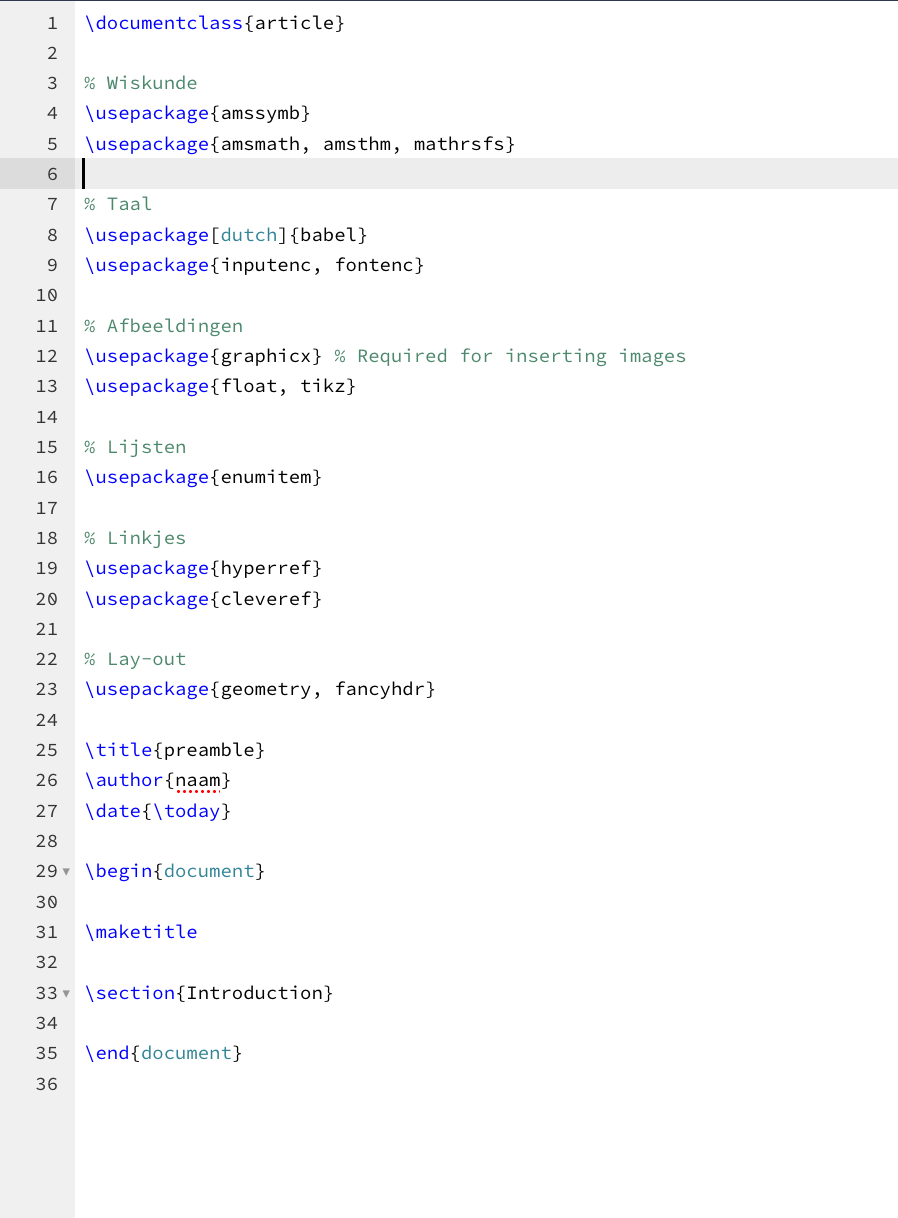
\includegraphics[width=0.45\linewidth]{./Images/preamble.png}
	\end{figure}
\end{frame}

\begin{frame}{Packages} 
	Handige packages zijn onder anderen:
	\begin{itemize}[label=\textbullet]
		\item \textbf{Voor wiskunde:} amssymb, amsmath, amsthm, mathrsfs
		\item \textbf{Voor taal:} babel, inputenc, fontenc
		\item \textbf{Voor afbeeldingen:} graphicx, float, tikz
		\item \textbf{Voor lijsten:} enumitem
		\item \textbf{Voor linkjes:} hyperref, cleveref
		\item \textbf{Voor lay-out:} geometry, fancyhdr
	\end{itemize}
\end{frame}

\begin{frame}[fragile, t]{Enumitem}
	\begin{columns}[t]
		% Om een of andere reden overlapten de columns en daarom heb ik hspace toegevoegd om het uit elkaar te halen. Ik kon helaas niet een betere oplossing vinden.
		\hspace{-0.6\textwidth}
		\begin{column}{0.6\textwidth}
			\begin{minted}{tex}
				Een genummerde lijst kan 
				gemaakt worden met
				\begin{enumerate}[label=\arabic*.]
					\item pen
					\item papier
					\item laptop
				\end{enumerate}
				en een ongenummerde lijst met
				\begin{itemize}[label=\textbullet]
					\item lunch
					\item waterfles
				\end{itemize}
			\end{minted}
			\par
		\end{column}
		% Weer een hspace om de tekst niet te laten overlappen
		\hspace{0.6\textwidth}
		\begin{column}{0.36\textwidth}
			\vspace{1mm}
			\cmfontblock{\small
				\noindent
				Een genummerde lijst kan gemaakt worden met
				\begin{enumerate}[label=\arabic*.]
					\item pen
					\item papier
					\item laptop
				\end{enumerate}
				en een ongenummerde lijst met
				\begin{itemize}[label=\textbullet]
					\item lunch
					\item waterfles
				\end{itemize}
			}
		\end{column}
		
	\end{columns} 
\end{frame}

\begin{frame}[fragile, t]{Enumitem (short labels)}
	\begin{columns}[t]
		% Weer een hspace om de tekst niet te laten overlappen
		\hspace{-0.6\textwidth}
		\begin{column}{0.6\textwidth}
			\begin{minted}{tex}
				Een genummerde lijst kan 
				gemaakt worden met
				\begin{enumerate}[1.]
					\item pen
					\item papier
					\item laptop
				\end{enumerate}
			\end{minted}
			\par
		\end{column}
		
		% Weer een hspace om de tekst niet te laten overlappen
		\hspace{0.6\textwidth}
		\begin{column}{0.36\textwidth}
			\vspace{2mm}
			\cmfontblock{ \small
				
				\noindent
				Een genummerde lijst kan gemaakt worden met
				\begin{enumerate}[1.]
					\item pen
					\item papier
					\item laptop
				\end{enumerate}
			}
		\end{column}
	\end{columns}
	\vspace{1cm}
	Hiervoor moet je enumitem als volgt in de preamble zetten: \begin{verbatim}
		\usepackage[shortlabels]{enumitem}
	\end{verbatim}
\end{frame}

\begin{frame}[fragile, t]{Hyperref en cleveref}
	\begin{columns}[t]
		% Weer een hspace om de tekst niet te laten overlappen
		\hspace{-0.6\textwidth}
		\begin{column}{0.6\textwidth}
			\begin{minted}{tex}
				Stel dat ik wil terug refereren naar 
				\begin{align}\label{eq: cirkel}
					x^2 + y^2 = a
				\end{align}
				dan kan ik nu gemakkelijk terug 
				refereren naar een formule 
				van de cirkel met \cref{eq: cirkel}.
				In plaats hiervan kan je
				ook \ref{eq: cirkel} gebruiken.
				Dit kan je ook doen 
				voor figuren, sections en meer.
			\end{minted}
			\par
		\end{column}
		
		% Weer een hspace om de tekst niet te laten overlappen
		\hspace{0.7\textwidth}
		\begin{column}{0.36\textwidth}
			\vspace{1mm}
			\cmfontblock{ \small
				
				\noindent
				Stel dat ik wil terug refereren naar 
				\begin{align}\label{eq: cirkel2}
					x^2 + y^2 = a
				\end{align}
				dan kan ik nu gemakkelijk terug 
				refereren naar een formule 
				van de cirkel met \cref{eq: cirkel2}.
				In plaats hiervan kan je ook \ref{eq: cirkel2} gebruiken.
				Dit kan je ook doen voor figuren, sections en meer.
			}
		\end{column}
	\end{columns}
	\vspace{0.5cm}
	Pas op: eerst hyperref in je preamble introduceren en daarna cleveref!
\end{frame}

\begin{frame}{Probeer het zelf}
	Probeer zelf eens: 
	\begin{enumerate}[label=\roman*.]
		\item een genummerde lijst te maken,
		\item een ongenummerde lijst te maken,
		\item een label te geven aan een section, figuur, stelling of iets anders,
		\item als je een label hebt, probeer er nu naar te refereren,
		%    \item pas de marges van je document aan.
	\end{enumerate}
\end{frame}